\documentclass{fenicscourse}

\begin{document}

\fenicslecture{Lecture 3: Static nonlinear PDEs}
              {Marie E. Rognes \\ Garth N. Wells}

% Variational problem
\begin{frame}
  \frametitle{The Stokes equations}

  We consider the stationary Stokes equations: find the velocity $u$
  and the pressure $p$ such that
  \begin{equation*}
    \begin{split}
      - \Div (2\nu \epsilon(u) - p \, \mathrm{I}) &= f \quad \mbox{in } \Omega \\
      \Div u &= 0 \quad \mbox{in } \Omega \\
    \end{split}
  \end{equation*}
  where $\epsilon(u) = \frac{1}{2}\left(\Grad u + (\Grad u)^{T}\right)$
  and with boundary conditions
  \begin{equation*}
    \begin{split}
      u &= 0 \quad \mbox{on } \partial \Omega_D \\
      - (2\nu \epsilon - p \, \mathrm{I}) \cdot n &= p_0 \, n
      \quad \mbox{on } \partial \Omega_N
    \end{split}
  \end{equation*}

  If viscosity $\nu$ varies with $u$ (or $p$),
  \begin{equation*}
    \nu = \nu(u)
  \end{equation*}
  this is a nonlinear system of partial differential equations.
\end{frame}

\begin{frame}[shrink=10]
  \frametitle{The Stokes equations: variational formulation}

  \medskip

  Assume that $u \in V$ and $p \in Q$, then $w = (u, p) \in V \times Q
  = W$. \\
  Let $f = 0$.

  \begin{block}{Step 1}
  Multiply by test functions $(v, q) \in W$ and integrate first
  equation by parts
  \begin{align*}
    \int_{\Omega} 2\nu \epsilon(u) \cdot \Grad v \dx
    - &\int_{\Omega} p \Div v \dx
    - \int_{\partial \Omega} (2\nu \epsilon(u)
    - p \, \mathrm{I}) \cdot n \cdot v \ds
    = 0 \\
    &\int_{\Omega} \Div u \, q \dx = 0
  \end{align*}
  \end{block}

  \vspace{-1em}

  \begin{block}{Step 2}
  Adding the equations and incorporating the boundary conditions we
  obtain: find $(u, p) \in W = V_0 \times Q$ such that
  \begin{align*}
    \int_{\Omega} 2\nu \epsilon(u) \cdot \Grad v \dx
    - \int_{\Omega} p \Div v \dx
    - \int_{\Omega} \Div u \, q \dx
    + \int_{\partial \Omega_N} p_0 \, v \cdot n \ds = 0
  \end{align*}
  for all $(v, q) \in W = V_0 \times Q$ where $V_0 = \{v \in V \,
  \text{such that} \, v |_{\partial \Omega_D} = 0 \}$.
  \end{block}

\end{frame}

\begin{frame}%[shrink=10]
  \frametitle{Canonical nonlinear variational problem}
  \bigskip

  The following canonical notation is used in FEniCS for (possibly)
  nonlinear problems:

  \bigskip

  \begin{columns}[t]
    \begin{column}{0.4\textwidth}
      Find $w \in W$ such that
      \begin{equation*}
        F(w; y) = 0
      \end{equation*}
      for all $y \in \hat{W}$.
    \end{column}
    \begin{column}{0.4\textwidth}
      \vspace{-2em}
      {\small
      \begin{block}{Note}
        Here, $w$ is a function, and $y$ is a test function, and so $F$ is
        a \emph{linear form}.
      \end{block}
      }
    \end{column}
  \end{columns}

  \bigskip
  \begin{block}{For the Stokes example}
  The functions are $w = (u, p)$, $y = (v, q)$ and the form $F$ is
  \begin{equation*}
    \begin{split}
    F(w; y) =
    &\int_{\Omega} 2\nu \epsilon(u) \cdot \Grad v \dx
    - \int_{\Omega} p \Div v \dx
    - \int_{\Omega} \Div u \, q \dx \\
    &+ \int_{\partial \Omega_N} p_0 \, v \cdot n \ds
    \end{split}
  \end{equation*}
  \end{block}
\end{frame}

\begin{frame}
  \frametitle{The Stokes equations introduce some new concepts}

  \begin{itemize}
  \item
    Mixed function spaces
  \item
    Integration over boundaries
  \item
    Solving nonlinear problems (if nonlinear viscosity)
  \item
    (Reading a mesh from file)
  \item
    (Adjusting parameters)
  \end{itemize}

\end{frame}


% Code step by step
\begin{frame}[fragile]
  \frametitle{Step by step: initializing a mesh from file}

  DOLFIN can read and write meshes from its own \emp{.xml} or
  \emp{.xml.gz} format
  \vspace{-1em}
  \begin{python}
mesh = Mesh("dolfin-1.xml.gz")
plot(mesh)
  \end{python}

  Conversion tools exist for other mesh formats
  \vspace{-1em}
  \begin{python}
$ man dolfin-convert
  \end{python}

  We will need the normal on the mesh boundary facets:
  \vspace{-1em}
  \begin{python}
n = FacetNormal(mesh)
  \end{python}

\end{frame}

\begin{frame}[fragile]
  \frametitle{Step by step: creating mixed function spaces}

  Mixed elements are created by taking the product of more basic elements
  \vspace{-1em}
  \begin{python}
# Define Taylor--Hood function space W
P2 = VectorElement("Lagrange", triangle, 2)
P1 = FiniteElement("Lagrange", triangle, 1)
TH = P2 * P1
#TH = MixedElement([P2, P1])
W = FunctionSpace(mesh, TH)
  \end{python}

  You can define functions on mixed spaces and split into components:
  \vspace{-1em}
  \begin{python}
w = Function(W)
(u, p) = split(w)
  \end{python}
  ... and arguments:
  \vspace{-1em}
  \begin{python}
y = TestFunction(W)
(v, q) = split(y)
# (v, q) = TestFunctions(W)
  \end{python}

\end{frame}

\begin{frame}[fragile]
  \frametitle{Step by step: more about defining expressions}

  Again, the pressure boundary value can be defined using an
  expression:
  \begin{python}
p0 = Expression("1 - a*x[0]", degree=1, a=2)
  \end{python}

  \bigskip

  When we specify the degree argument, this will be used as the
  polynomial degree when the expression is used in forms. Otherwise,
  the degree will be estimated heuristically.

  \bigskip

  All parameters (in this case \emp{a}) must be specified at
  initialization, and can be modified later

\end{frame}

\begin{frame}[fragile, shrink=5]
  \frametitle{FAQ: What is the difference between a \emp{Function} and an \emp{Expression}?}

 \begin{block}{Function}
   ... is described by expansion coefficients with
   reference to a \emp{FunctionSpace} with a given basis:
   $u = \sum_{i} u_i \phi_i$
   \vspace{-1em}
   \begin{python}
u = Function(V) # Defines the function space
u.vector()      # The coefficients
   \end{python}

 \end{block}
 \begin{block}{Expression}
   ... given by an evaluation formula (more or less explicit)
   \vspace{-1em}
   \begin{python}
f = Expression("...", degree=...)

class Source(Expression):
    def eval(self, values, x)
        ...
   \end{python}
 \end{block}

 During \emp{assemble} an \emp{Expression} is interpolated into a
 polynomial space of the given degree on each cell.

\end{frame}


\begin{frame}[fragile]
  \frametitle{Step by step: defining the viscosity}

We may want to play with different viscosities.

\bigskip

In the simplest case, it is just constant: $\nu = 0.1$
\vspace{-1em}
  \begin{python}
nu = 0.1
  \end{python}

... or it can vary with the domain: $\nu = 1 + 100 x_1$
\vspace{-1em}
  \begin{python}
nu = Expression("1 + 100*x[1]", degree=1)
  \end{python}

... or it can vary with the unknown: $\nu = (u \cdot u)^{1/2}$
\vspace{-1em}
  \begin{python}
w = Function(W)
(u, p) = split(w)
def viscosity(u):
    return inner(u, u)**(1./2)
nu = viscosity(u)
  \end{python}

\end{frame}

\begin{frame}[fragile]
  \frametitle{Step by step: defining a boundary condition on a subspace}

  Assume that we have a mixed function space:
  \vspace{-1em}
  \begin{python}
W = FunctionSpace(mesh, V * Q)
  \end{python}

\bigskip

The subspaces of W can be retrieved using \emp{sub}:
  \vspace{-1em}
  \begin{python}
W0 = W.sub(0)
  \end{python}
Note that \emp{W0} is not completely the same as \emp{V}

\bigskip

  The following code defines a homogenous Dirichlet (boundary)
  condition on the first subspace at the part where $x_0 = 0$.
  \vspace{-1em}
  \begin{python}
g = (0.0, 0.0)
bc = DirichletBC(W.sub(0), g, "near(x[0], 0.0)")
  \end{python}
\end{frame}


\begin{frame}[fragile, shrink=5]
  \frametitle{Stokes: defining the variational form}

  Assume that we have
\vspace{-1em}
  \begin{python}
w = Function(W)
(u, p) = split(w)
(v, q) = TestFunctions(W)
p0 = ...; nu = ...; n = ...
  \end{python}

  We can now specify the linear form $F$
  \vspace{-1em}
  \begin{python}
epsilon = 2*sym(grad(u))
F = (nu*inner(epsilon, grad(v)) \
    - div(u)*q - div(v)*p)*dx \
    + p0*dot(v, n)*ds
  \end{python}

\bigskip

Note that \emp{dx} denotes integration over cells, \emp{ds} denotes
integration over exterior (boundary) facets, \emp{dS} denotes
integration over interior facets.

\bigskip

\alert{FAQ:} How to specify integration over only subdomains?
See the \emph{Poisson with multiple subdomains} demo.

\end{frame}

\begin{frame}[fragile]
  \frametitle{Step by step: solving (nonlinear) variational problems}

  Once a variational problem has been defined, it may be solved
  by calling the \emp{solve} function (as for linear problems):
\vspace{-1em}
  \begin{python}
solve(F == 0, w, bc)
  \end{python}

Or more verbosely
\vspace{-1em}
  \begin{python}
dF = derivative(F, w)
pde = NonlinearVariationalProblem(F, w, bc, dF)
solver = NonlinearVariationalSolver(pde)
solver.solve()
  \end{python}

Extracting the subfunctions (as DOLFIN functions)
\vspace{-1em}
  \begin{python}
(u, p) = w.split(deepcopy=True)
  \end{python}



\end{frame}

\begin{frame}[fragile]
  \frametitle{Step by step: adjusting parameters in DOLFIN}

  \bigskip

  Adjusting global parameters
\vspace{-1em}
  \begin{python}
from fenics import *
info(parameters, True)
parameters["form_compiler"]["cpp_optimize"] = True
#parameters["form_compiler"]["optimize"] = True
  \end{python}

  \bigskip

  Adjusting local (and nested) parameters
\vspace{-1em}
  \begin{python}
solver = NonlinearVariationalSolver(pde)
info(solver.parameters, True)
solver.parameters["symmetric"] = True
solver.parameters["newton_solver"]["maximum_iterations"] = 100
  \end{python}
\normalsize

\end{frame}

\begin{frame}[fragile, shrink=40]
\frametitle{Stokes: a complete code example}
\inputanycode{src/03_static_nonlinear_pdes/apa/stokes_example.py}
\end{frame}

\begin{frame}[fragile]
\frametitle{Stokes: running the example yields}
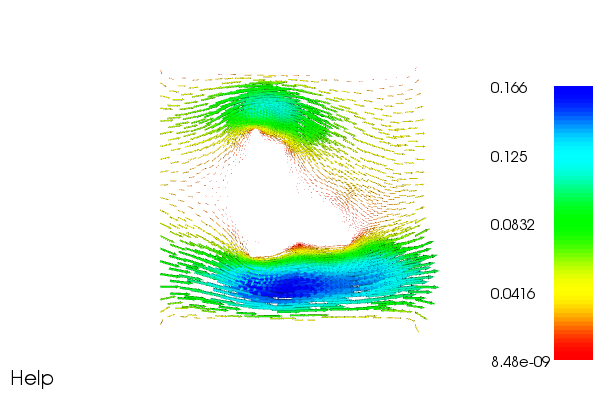
\includegraphics[width=0.5\textwidth]{png/velocity.png}
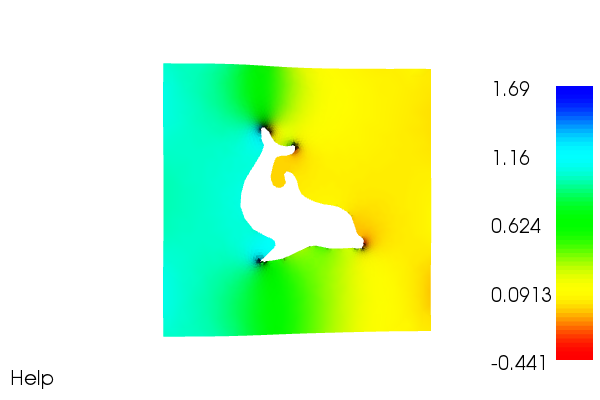
\includegraphics[width=0.5\textwidth]{png/pressure.png}
\begin{python}
  $ python stokes_example.py
\end{python}
\end{frame}


\begin{frame}
  \frametitle{\emph{FEniCS programming challenge!}}
  \bigskip

  Solve the Stokes problem on $\Omega$ defined by the \emp{dolfin-1.xml.gz} mesh,
  defined by the following data
  \begin{equation*}
    \begin{split}
      - \Div (2\nu \epsilon(u) - p \, \mathrm{I}) = 0 \quad &\text{in } \Omega \\
      \Div u = 0 \quad &\text{in } \Omega \\
      - (2\nu \epsilon(u) - p \, \mathrm{I}) \cdot n = p_0 \, n
      \quad &\text{on } \partial \Omega_N = \{(x_0, x_1) | \, x_0 = 0 \text{ or } x_0 = 1\} \\
      p_0 = 1 - x_0 \quad & \\
      u = 0 \quad & \text{on } \partial \Omega_D = \partial \Omega \backslash \partial \Omega_N
    \end{split}
  \end{equation*}

  \begin{enumerate}
  \item[Ex.~1] Consider a constant viscosity $\nu = 0.2$, plot the
    solutions.
  \item[Ex.~2] Consider the nonlinear viscosity
    \begin{equation*}
      \nu = \nu(u) = 0.5 (\Grad u \cdot \Grad u)^{1/(2 (n-1))}, n = 4
    \end{equation*}
    Plot the solutions and estimate the \alert{average velocity} in
    the $x[0]$-direction.
  \end{enumerate}

  {\tiny \alert{Hint}: For Ex. 2, you may need to compute an approximation
    first in order to provide a suitable initial guess to the Newton
    solver}

\end{frame}


\end{document}
